\documentclass[12pt]{article}
\usepackage{amsmath}
\usepackage{graphicx}
\usepackage{hyperref}
\usepackage{listings}
\usepackage{color}
\usepackage{pythonhighlight}

\title{Operating System Course Report - First Half of the Semester}
\author{B class}
\date{\today}

\begin{document}

\maketitle
\newpage

\tableofcontents
\newpage

\section{Introduction}
This report summarizes the topics covered during the first half of the Operating System course. It includes theoretical concepts, practical implementations, and assignments. The course focuses on the fundamentals of operating systems, including system architecture, process management, CPU scheduling, and deadlock handling.

\section{Course Overview}
\subsection{Objectives}
The main objectives of this course are:
\begin{itemize}
    \item To understand the basic components and architecture of a computer system.
    \item To learn process management, scheduling, and inter-process communication.
    \item To explore file systems, input/output management, and virtualization.
    \item To study the prevention and handling of deadlocks in operating systems.
\end{itemize}

\subsection{Course Structure}
The course is divided into two halves. This report focuses on the first half, which covers:
\begin{itemize}
    \item Basic Concepts and Components of Computer Systems
    \item System Performance and Metrics
    \item System Architecture of Computer Systems
    \item Process Description and Control
    \item Scheduling Algorithms
    \item Process Creation and Termination
    \item Introduction to Threads
    \item File Systems
    \item Input and Output Management
    \item Deadlock Introduction and Prevention
    \item User Interface Management
    \item Virtualization in Operating Systems
\end{itemize}

\section{Topics Covered}

\subsection{Basic Concept455555555555555545s and Components of Computer Systems}
    \subsubsection{Definisi dan Konsep}
    \subsubsection{Komponen-Komponen Sistem Komputer}
    Sistem komputer merupakan kesatuan yang terbentuk dari beberapa komponen utama yang saling berhubungan untuk menjalankan fungsi komputasi. Ketiga komponen utama tersebut adalah hardware, software, dan brainware. Kombinasi ketiganya memungkinkan komputer untuk melakukan berbagai tugas, mulai dari pengolahan data, penyimpanan informasi, hingga eksekusi perintah.
    \begin{itemize}
        \item Hardware
        \par
        Hardware adalah perangkat keras mengacu pada perangkat fisik yang dapat dilihat dan disentuh, seperti CPU, monitor, keyboard, dan komponen internal lainnya. Hardware berperan sebagai fondasi yang menyediakan platform untuk berjalannya software. Perangkat keras pada sistem komputer terbagi atas 3 bagian, yaitu:
        \begin{itemize}
            \item Input Unit
            \par 
            Input unit merupakan bagian dari perangkat keras yang berfungsi sebagai alat untuk memasukkan data dan lainnya ke dalam komputer. Perangkat input unit antara lain, keyword, mouse, camera digital, dan sebagainya.
            \item Processing Unit
            \par
            Processing unit biasanya disebut CPU (\textit{Central Processing Unit}) yang merupakan otak atau jantung dari komputer karena mengendalikan semua fungsi yang terjadi dalam sistem komputer. Perangkat utamanya berupa prosesor dan chipset yang biasanya terdapa pada \textit{motherboard}. CPU memiliki 3 komponen utama, yaitu:
            \begin{itemize}
                \item Arimatic dan Logical Unit (ALU)
                \par
                ALU bertugas untuk melakukan perhitungan yang bersifat arimatik dan melakukan keputusan dari operasi logika dan manipulasi bit sesuai dengan instruksi program
                \item Control Unit
                \par
                Control unit berfungsi sebagai pengatur dan pengendali semua peralatan yang ada pada sistem komputer dan mengatur kapan alat input menerima data dan kapan menampilkan output di monitor
                \item Main Memory
                \par
                Main memory merupakan tempat atau media yang digunakan untuk menyimpan data yang akan atau sedang dikelola oleh sistem komputer. Main memory terbagi menjadi 2, yaitu:
                \begin{itemize}
                    \item ROM (\textit{Read Only Memory})
                    \par
                    ROM merupakan memori permanen yang terdapat di dalam sistem komputer yang sudah disusun atau sudah dibuat dipabrik pembuatan dan biasanya tidak bisa diubah oleh user komputer.
                    \item RAM  (\textit{Random Access Memory})
                    \par
                    RAM adalah memori yang memuat semua data yang dimasukkan melalui alat input pada setiap aplikasi yang akan dimasukkan terlebih dahulu ke dalam memori main dan RAM ini biasanya bersifat sementara karena apabila komputer dimatikan maka semua data tersebut akan hilang.
                \end{itemize}
            \end{itemize}
        \item Output Unit 
        \par
        Output unit merupakan perangkat keras yang berfungsi untuk menyajikan output dari proses yang sedang dikerjakan pada komputer. Bentuk peralatan output ini antara lain, monitor, printer, projector, speaker, dan lain-lain.
        \end{itemize}
        
        \item Software 
        \par
        Software adalah perangkat lunak atau program yang berjalan di atas hardware. Software bertugas mengendalikan dan mengatur hardware agar dapat bekerja sesuai dengan fungsi yang diinginkan, seperti sistem operasi, aplikasi, dan program utilitas. Perangkat lunak menjembatani interaksi user dengan komputer yang hanya memahami bahasa komputer. Secara umum, perangkat lunak terbagi menjadi 2, yaitu
        \begin{itemize}
            \item Operation System Software
            \par
            Operation System Software merupakan perangkat lunak yang memiliki fungsi untuk mengonfigurasikan komputer agar menerima berbagai perintah dasar yang diberikan untuk dimasukkan. Contohnya, Linux, MS-DOS, dan lain-lain
            \item Perangkat Lunak Aplikasi
            \par
            Perangkat Lunak Aplikasi merupakan program yang siap pakai yang digunakan di suatu bidang tertentu, seperti aplikasi pada bisnis dan perkantoran yang biasanya menggunakan\textit{ Microsoft Office, Koffice}, dan lain-lain
        \end{itemize}
        \item Brainware 
        \par
        Brainware mencakup pengguna atau orang yang berinteraksi dengan komputer, baik itu sebagai pengguna akhir, pengembang, maupun administrator. Brainware berperan dalam merancang, mengoperasikan, dan memanfaatkan teknologi komputer secara optimal.
    \end{itemize}
   

\subsection{System Performance and Metrics}
This section introduces various system performance metrics used to measure the efficiency of a computer system, including throughput, response time, and utilization.

\subsection{System Architecture of Computer Systems}
Describes the architecture of modern computer systems, focusing on the interaction between hardware and the operating system.

\subsection{Process Description and Control}
Processes are a central concept in operating systems. This section covers:
\begin{itemize}
    \item Process states and state transitions
    \item Process control block (PCB)
    \item Context switching
\end{itemize}

\subsection{Scheduling Algorithms}
This section covers:
\begin{itemize}
    \item First-Come, First-Served (FCFS)
    \item Shortest Job Next (SJN)
    \item Round Robin (RR)
\end{itemize}
It explains how these algorithms are used to allocate CPU time to processes.

\subsection{Process Creation and Termination}
Details how processes are created and terminated by the operating system, including:
\begin{itemize}
    \item Process spawning
    \item Process termination conditions
\end{itemize}

\subsection{Introduction to Threads}
This section introduces the concept of threads and their relation to processes, covering:
\begin{itemize}
    \item Single-threaded vs. multi-threaded processes
    \item Benefits of multithreading
\end{itemize}

\begin{figure}[h]
    \centering
    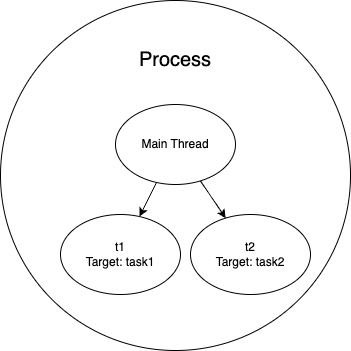
\includegraphics[width=0.5\textwidth]{/Users/khawaritzmi/Unhas/os_report_mid2024/b_class/asset/example.png}  % Sesuaikan nama file dan ukurannya
    \caption{Ini adalah gambar contoh dari multithreading.}
    \label{fig:contoh_gambar}
\end{figure}

Seperti yang terlihat pada Gambar \ref{fig:contoh_gambar}, inilah cara menambahkan gambar dengan keterangan.

\subsection{File Systems}
File systems provide a way for the operating system to store, retrieve, and manage data. This section explains:
\begin{itemize}
    \item File system structure
    \item File access methods
    \item Directory management
\end{itemize}

\subsection{Input and Output Management}
Input and output management is key for handling the interaction between the system and external devices. This section includes:
\begin{itemize}
    \item Device drivers
    \item I/O scheduling
\end{itemize}

\subsection{Deadlock Introduction and Prevention}
Explores the concept of deadlocks and methods for preventing them:
\begin{itemize}
    \item Deadlock conditions
    \item Deadlock prevention techniques
\end{itemize}

\subsection{User Interface Management}
This section discusses the role of the operating system in managing the user interface. Topics covered include:
\begin{itemize}
    \item Graphical User Interface (GUI)
    \item Command-Line Interface (CLI)
    \item Interaction between the user and the operating system
\end{itemize}

\subsection{Virtualization in Operating Systems}
Virtualization allows multiple operating systems to run concurrently on a single physical machine. This section explores:
\begin{itemize}
    \item Concept of virtualization
    \item Hypervisors and their types
    \item Benefits of virtualization in modern computing
\end{itemize}

\section{Assignments and Practical Work}
\subsection{Assignment 1: Process Scheduling}
Students were tasked with implementing various process scheduling algorithms (e.g., FCFS, SJN, and RR) and comparing their performance under different conditions.
\subsubsection{Group 1}
\begin{python}
    class Process:
    def __init__(self, pid, arrival_time, burst_time):
        self.pid = pid
        self.arrival_time = arrival_time
        self.burst_time = burst_time
        self.completion_time = 0
        self.turnaround_time = 0
        self.waiting_time = 0
\end{python}

\begin{table}[htbp] % Optional: For floating position
    \centering
    \begin{tabular}{|c|c|c|} % Defines number of columns and alignment (c = center, l = left, r = right). '|' creates vertical lines.
    \hline
    Header 1 & Header 2 & Header 3 \\ % Column headers
    \hline
    Row 1, Column 1 & Row 1, Column 2 & Row 1, Column 3 \\ % First row of data
    \hline
    Row 2, Column 1 & Row 2, Column 2 & Row 2, Column 3 \\ % Second row of data
    \hline
    \end{tabular}
    \caption{Your table caption} % Optional: For adding a caption
    \label{tab:your_label} % Optional: For cross-referencing the table
\end{table}

\subsection{Assignment 2: Deadlock Handling}
In this assignment, students were asked to simulate different deadlock scenarios and explore various prevention methods.

\subsection{Assignment 3: Multithreading and Amdahl's Law}
This assignment involved designing a multithreading scenario to solve a computationally intensive problem. Students then applied **Amdahl's Law** to calculate the theoretical speedup of the program as the number of threads increased.

\subsection{Assignment 4: Simple Command-Line Interface (CLI) for User Interface Management}
Students were tasked with creating a simple **CLI** for user interface management. The CLI should support basic commands such as file manipulation (creating, listing, and deleting files), process management, and system status reporting.

\subsection{Assignment 5: File System Access}
In this assignment, students implemented file system access routines, including:
\begin{itemize}
    \item File creation and deletion
    \item Reading from and writing to files
    \item Navigating directories and managing file permissions
\end{itemize}

\section{Conclusion}
The first half of the course introduced core operating system concepts, including process management, scheduling, multithreading, and file system access. These topics provided a foundation for more advanced topics to be covered in the second half of the course.

\end{document}